\chapter{Pruebas de concepto}
\section{Propuestas}
Una vez se han testeado y analizado las diferentes tecnologías surgen diferentes ideas como prueba de concepto en función de las características particulares de cada tecnología. Las cuales son enumeradas a continuación:

\begin{itemize}
\item Desarrollo de un \textit{plugin} capaz de gestionar los \textit{cloud anchor} en interiores y almacenar la información durante un período de tiempo ajustable a las necesidades del producto. Será capaz de identificar estas posiciones \textit{online} y \textit{offline} mediante una base de datos almacenada tanto en servidor como en local si fuese necesario. Plataformas deseables: Android (prioritario) y iOS. 
\item API de alto nivel que permite desarrollar de manera más versátil y sencilla aplicaciones en realidad aumentada teniendo compatibilidad plena entre ARKit y ARCore. El usuario será capaz de desarrollar una aplicación en realidad aumentada completa sin apenas líneas de código ya sea mediante \textit{blueprints} o módulos.
\item Juego multijugador con \textit{Cloud Anchors}. Juego en el que dos jugadores o más compiten por conseguir más puntos por destruir edificios. (Inspirado en Bombardero - Amstrad CPC)
\item Plataforma de realidad aumentada: permitirá al usuario acceder en el momento a diferentes contenidos ya sean vídeos, juegos o experiencias sin necesidad de salir de la aplicación. Esta idea estaba pensada para el uso con unas gafas de AR y mando inalámbrico para el control del dispositivo. Inspirado en Google DayDream.
\item Reconocimiento de objetos.
\item Proceso de montaje de muebles paso a paso del en realidad aumentada.
\end{itemize}

\clearpage
\section{Juego multijugador con cloud anchor (ARCore) - BombARdero+}
La tecnlogía que mas nos ha impresionado ha sido los Cloud Anchors, nunca habíamos oído hablar de ella. Cuando nos enteramos de su existencia, estábamos todos de acuerdos en desarrollar un videojuego multijugador online.\\

Los Cloud Anchors, como hemos explicado anteriormente, se almacenan en la nube de Google. Para usarlos, hace falta conseguir una clave de licencia de \textit{ARCore Cloud Anchor API} en Google Cloud Platform \cite{GCloud}. Una vez conseguida la credencial, hay que introducirla en Unity3D, ``Edit -> Project Settings -> Google ARCore -> Cloud Anchor API Keys ''. En los ejemplos que ofrece Google, la implementación de los Cloud Anchor utiliza la \textit{Multiplayer High Level API(Multiplayer HLAPI)} de Unity, por lo que también hay que activar el servicio de multijugador en nuestro proyecto desde el \textit{dashboard} de Unity \cite{UnityDashboard}. Una vez realizado estos dos pasos, al compilar la escena de ejemplo, debería funcionar. En esa escena, un usuario tiene que crear una sala e instanciar un objeto, el punto de anclaje principal, que se convertirá en las coordenadas (0,0,0) del entorno.
Este punto de anclaje tarda unos diez segundos en subirse a la nube y estar disponible para más usuarios, que al entrar a la aplicación le aparece un listado con las salas disponibles. \\

Para desarrollar este juego, primero desarrollamos dos aplicaciones anteriormente.

Como al principio no teníamos dos móviles que soportasen ARCore, programamos el juego en monojugador, para acostumbrarnos al entorno y para ahorrarnos trabajo en un futuro.\\

En paralelo, como teníamos que implementar la parte de multijugador online y no teníamos ningún tipo de experiencia, realizamos unas pruebas para estudiar el funcionamiento de la Multiplayer HLAPI. Esas pruebas nos permitieron entender y aprender a desarrollar el multijugador de la prueba de concepto que nos hemos puesto como objetivo.\\

Una vez que conseguimos tener dos dispositivos que soportasen ARCore, empezamos a desarrollador la aplicación multijugador. Gracias a haber desarrollado el \textit{BombARdero}, nos permitió avanzar muy rápido ya que estaban los modelos, \textit{prefabs}\footnote{ Objetos prefabricados de Unity3d}, y scripts con las mecánicas básicas ya creadas. Primero tuvimos que mirar como estaba montada la implementación de Google, para entender el proceso de cómo se subía el marcador a la nube y la cantidad de información de control que teníamos. Este proceso fue bastante sencillo, ya que el código de ejemplo es muy entendible e intuitivo. Una vez conseguido implementar el BombARdero con los Cloud Anchor, hubo que hacer unos pequeños retoques a los scripts e añadir componentes a los objetos, para implementar la parte multijugador.\\
Continuará...


\clearpage
\section{Instrucciones de montaje de muebles en AR - AmueblAR}

En nuestra investigación hemos visto que una de las utilidades más populares actualmente en el campo de la realidad aumentada son las aplicaciones de decoración de interiores. Ikea, por ejemplo, ha lanzado Ikea Place, una aplicación de realidad aumentada para dispositivos móviles que permite visualizar cualquier habitación de tu casa con muebles virtuales. De esta manera podemos decidir si encajan con nuestro salón y si las medidas son las adecuadas para después comprar el mueble en la tienda física.\\

Este programa despertó nuestra curiosidad y pensamos que podríamos desarrollar una aplicación con una utilidad parecida, pero en este caso aplicada al montaje de los muebles. Sabemos que comprar sofás o estanterías por piezas es en ocasiones más barato y facilita enormemente el transporte, sin embargo la parte en la que muchos compradores experimentan problemas es a la hora de montarlos. Muchos son incapaces de ver en el plano de las instrucciones en qué lugar va cada tornillo o de qué forma se unen las patas. Por eso, la aplicación que nosotros hemos propuesto consiste en un pequeño manual de instrucciones en realidad aumentada sin marcadores. De esta manera se puede ver en todo momento el modelo 3D del mueble, rotarlo y además desplazarte alrededor de él para apreciar en detalle cada uno de los pasos en el proceso de montaje.\\

El funcionamiento es muy sencillo: para empezar escaneamos el plano para que el programa cree una superficie donde colocar el mueble. A continuación tocamos la pantalla en el lugar en el que queremos colocarlo. Ahora podemos rotar el mueble hacia izquierda y derecha para dejarlo en una posición en la que nos resulte cómodo acercarnos y alejarnos mientras vemos los pasos de montaje. Finalmente, al pulsar el botón de aceptar entramos en la fase de construcción. En ella tenemos un botón a cada lado de la pantalla: el de la izquierda retrocede al paso anterior y el de la derecha avanza al paso siguiente. Mientras se suceden las animaciones que van explicando cómo armar progresivamente el mueble el usuario puede moverse libremente con su dispositivo para apreciar los detalles e incluso retroceder si no ha entendido bien el paso a seguir.\\

Para el desarrollo hemos utilizado la librería ARCore, que permite el despliegue de realidad aumentada sin marcadores. Utilizando la tecnología que nos vienen dada por la librería buscamos una serie de puntos en el suelo que nos permitirán crear un plano virtual. Una vez generada esta superficie el plano se representa gráficamente en pantalla con la unión de los puntos. A continuación dividimos la aplicación en tres estados: despliegue, rotación y montaje.\\ 

Empezamos en la fase de despliegue, en la que el programa está continuamente esperando la interacción del usuario. Cuando se toca la pantalla, se comprueba si ha habido colisión con el plano virtual, y de ser así se instancia el mueble en el lugar en el que hemos tocado. Si este proceso se ha llevado a cabo con éxito, pasamos a la fase de rotación. Aquí aparecen dos botones azules a los lados de la pantalla y uno verde en la parte inferior. Los botones laterales llevan una referencia al mueble para que al ser pulsados lo roten en una u otra dirección. El botón inferior por otra parte nos sirve para comunicarle a la aplicación que estamos conformes con la posición actual del objeto y que puede pasar a la siguiente fase.\\ 

Finalmente nos encontramos con dos nuevos botones a los laterales, que como hemos explicado anteriormente se encargan de adelantar y retroceder los pasos de montaje. El sofá tiene un componente Animator Controller que lleva el árbol de estados. Este árbol consta de 10 estados fijos, en los que se queda el mueble una vez ha terminado su animación correspondiente y 18 estados móviles o animaciones, que se reproducen cuando pulsas el botón de avanzar o retroceder. Para ello, existe una variable que controla el avance y otra que hace lo propio con el retroceso, que se anulan una vez se entra en un estado estático y se activan al pulsar el botón que corresponde, pasando así a la animación del paso siguiente o anterior.\\

Cabe destacar el proceso de creación del mueble en sí mismo, que en el caso del ejemplo se trata del sofá Kivik(FOTO). Como no era posible encontrar un modelo dividido en piezas y fácilmente animable tuvimos que modelarlo desde cero con la ayuda de la documentación que encontramos en la web de Ikea. El mueble consta de las siguientes piezas: el asiento del sofá, el respaldo del sofá, el asiento de la \textit{cheslong} \footnote{ Tipo de sofá que posee una prolongación lo suficientemente larga en forma de L como para soportar las piernas humanas.} y su respaldo, los dos brazos, dos escuadras, una pletina, ocho patas, dieciocho tornillos con sus correspondientes tuercas y arandelas, cinco cojines cuadrados y un cojín alargado para la cheslong. Salvando los tornillos, de los que encontramos en una página de recursos gratuitos \cite{tornillos}, todos los demás fueron creados por nosotros en Blender, herramienta de la que ya hemos hablado anteriormente. Una vez terminadas las piezas del sofá, las texturizamos con colores azules y aspecto de sofá, teniendo las piezas como los tornillos o las escuadras una textura metálica.\\

Pensamos que podríamos empezar a animar cada parte por separado dentro de un objeto conjunto del que fueran hijas todas las piezas, pero para que Unity pueda interpretar cada acción como propia de un objeto mayor a las partes es necesario hacer un \textit{rigging}\footnote{ Proceso de crear un sistema de controles digitales y agregárselos a un modelo 3D para que así pueda ser animado fácilmente y eficientemente} que abarque todas piezas del sofá. Una vez construido el esqueleto hay que asignarle a cada hueso el objeto que se va a encargar de mover, lo cual dio también algunos problemas, ya que al tratarse de un objeto conjunto ciertos huesos acababan emparentándose automáticamente con partes del sofá que nos les correspondían, de modo que la única solución fue establecer manualmente los pesos (es decir, la influencia que tiene cada hueso sobre una parte concreta) sobre los diferentes conjuntos de vértices hasta que conseguimos el resultado que esperábamos.\\

En lo referente a las animaciones nos fue muy útil el vídeo que tiene publicado la cuenta de Ikea España en la plataforma Youtube \cite{IkeaYT} en el que se explica el procedimiento que se sigue para construir el sofá. Habiéndolo analizado dividimos el montaje en 9 pasos diferenciados y los animamos también en Blender, haciendo desaparecer las partes que no se están utilizando en ese momento para que sea más claro y fácil verlo.\\

Al contrario que en los ejemplos con marcadores en los que pudimos exportar directamente el archivo de Blender para su uso en Unity, aquí nos dio problemas ya que el editor dejó de reconocer los clips de vídeo de algunas animaciones. Solventamos este problema exportando el objeto desde el programa de modelado en formato fbx, pero nos surgió otro nuevo inconveniente: todas las partes del sofá habían perdido sus texturas. Ya desde Unity creamos los materiales por separado y se los asignamos a cada pieza.
Fue un proceso bastante agotador, sobre todo en la parte artística, pero consideramos que el resultado es satisfactorio y útil, además ofrece nuevas posibilidades en un campo que no deja de crecer.

\clearpage
\section{Visualizador de objetos en AR con gafas Aryzon (ARCore)}
En la fase de investigación, pensamos que una de las limitaciones de la realidad aumentada en dispositivos móviles es el hecho de tener que que estar sujetando el móvil con las manos, por lo que el control y la experiencia de usuario se ve condicionada negativamente. Decidimos buscar un headset de realidad aumentada encontramos las gafas de Aryzon \cite{Aryzon}, compramos un ejemplar y probamos qué tal funcionaban.\\

Descargamos las aplicaciones y juegos que promocionan para ver como era la experiencia usando las gafas. Nos resultó curioso y decidimos desarrollar una aplicación en la que se pudiera ver objetos y/o modelos 3D y poder caminar alrededor de ellas. Para añadirle más funcionalidad, usamos un mando de \textit{Xbox One} que nos permitirá mover, rotar y escalar el modelo a nuestro gusto, con el objetivo de poder manipular la aplicación sin necesidad de tocar el móvil, ya que éste estará colocado en las gafas.\\

Para el desarrollo de la aplicación usamos el SDK de Aryzon, que nos facilita la vista estereoscópica\footnote{ Dos puntos de vista poco separados entre sí} para simular nuestros ojos, ya que las gafas están compuestas por dos espejos que reflejan la imagen al cristal por donde nosotros vemos el mundo real, permitiendo tener esa visión de realidad aumentada como se puede observar en la figura \ref{GafasAryzon}.

\begin{figure}[H]
    \centering
    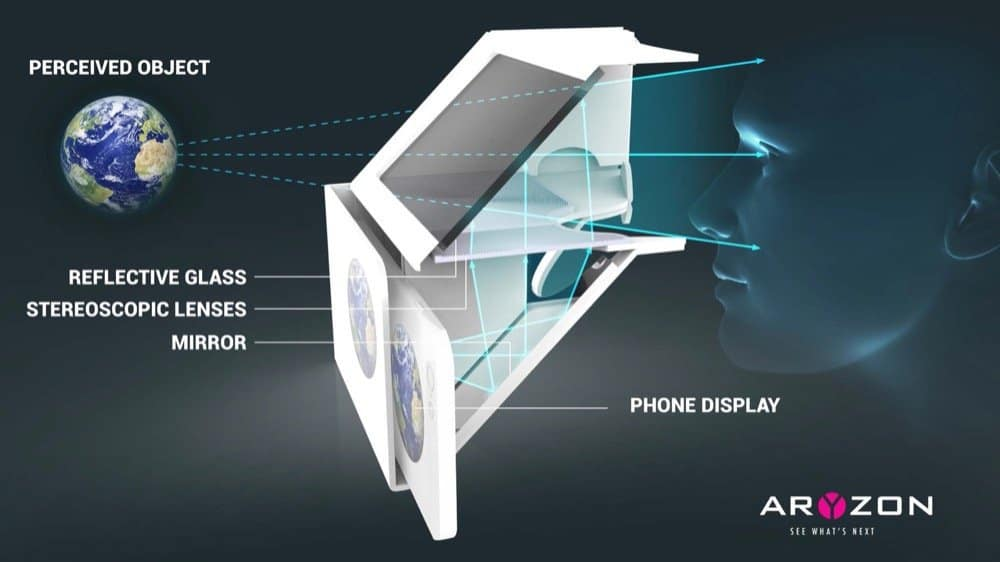
\includegraphics[width=0.5\linewidth]{Images/How-it-works.jpg}
    \caption{Como funciona las gafas de Aryzon. Imagen sacada de (\url{https://www.igadgetsworld.com/aryzon-diy-augmented-reality-headset/}}
    \label{GafasAryzon}
\end{figure}


Todos los ejemplos que proporciona Aryzon son con marcadores o no usan de verdad realidad aumentada, si no que que es una escena de realidad virtual con fondo negro y vista esteoroscópica, entonces da el efecto de ser realidad aumentada, pero la aplicación en sí es realidad virtual. Nosotros hemos decidido usar ARCore, ya que queremos usar la realidad aumentada sin marcadores y movernos alrededor del modelo, y como hemos visto en las pruebas, la estabilidad de los puntos de anclaje de ARCore funcionan muy bien.\\
Continuará...

\noindent